\documentclass[a4paper]{IEEEtran}

\usepackage[backend=bibtex]{biblatex}
\addbibresource{paper}
\usepackage{hyperref}
\usepackage{graphicx}
\usepackage{amsmath,amsfonts}
\usepackage{algorithm,algorithmicx,algpseudocode}
\renewcommand{\algorithmicrequire}{\textbf{Input:}}
\renewcommand{\algorithmicensure}{\textbf{Output:}}

\title{Locating Data Flow Anomaly With Statistical Distance}
\author{Ruoyu Wang}
\date{2017.05.04}

\begin{document}
	\maketitle
	
	\begin{abstract}
		[abstract]
	\end{abstract}
	
	\section{Introduction}
		Big data industry has been blooming within this decade, reshaping the form of life and work across the globe. According to~\autocite{letouze2014official}, 1.2ZB data had been produced from 2012 to 2014. And the amount doubles every two years. Currently, there are totally 2.7ZB data in the digital universe~\autocite{bigDataStatistics}. Big data analysis has been widely adopted in scientific experiments~\autocite{nothaft2015rethinking}, electric business~\autocite{bronson2015open,sumbaly2013big,chen2016realtime}, healthcare~\autocite{groves2016big}, governments~\autocite{kim2014big} and many other fields.
		
		However, it will be harder in the future to harness the exploding volumes of data since problems have already appeared in data management and engineering, threatening trustworthiness and reliability of data flows inside working systems. Data error rate in enterprises is approximately 1\% to 5\%, and for some, even above 30\%~\autocite{saha2014data}.
		
		Those data anomalies may arise due to both internal and external reasons with respect to a certain system. From one hand, components inside the system may generate problematic source data. For example, in a sensor network, some sensors may generate erroneous data when it experiences power failure or other extreme conditions~\autocite{rassam2014adaptive}. Data packages will be lost if sensor nodes fail to connect to network or some sensor hub goes down~\autocite{herodotou2014scalable}. Also, human operators act as a heavily vulnerable part to bugs and mistakes. Some even deliberately modify system configurations for malicious compromises~\autocite{schuster2015vc3}. A study~\autocite{humanError} found that 65\% of organizations state that human errors are the main  cause of data problems.
		
		On the other hand, data manipulation~\autocite{dataManipulation} from outside hackers composes another potential threat of data quality and reliability. Taken Apache Hadoop as an example. It's security issues has long been discussed within communities and industry~\autocite{sharif2015current,terzi2015survey,jam2014survey,sharma2014securing}. As is shown in Figure~\ref{fig:hadoop-security}, the two basic vulnerabilities: \textit{lack of access control} and the \textit{absence of encryption} expose the entire cluster to dangerous threats. Data flows can be intercepted and modified; services can also be altered and blocked~\autocite{huang2014denial}. Although there are several frameworks(e.g. Kerberos, Sentry, Knox etc.) and algorithms providing basic protection~\autocite{zheng2017towards,sikdar2017spatio,xu2016high,yu2015enhancing,cohen2014towards}, clever attackers can always bypass the barriers and sneak into the core of data pipelines. Several approaches are developed as sentinels to detect probable infiltrations. However, these approaches are not able to locate corrupted data under carefully planned manipulations. Nor can they figure out the exact reasons and recover the original records. To locate and diagnose anomalies in data pipelines under carefully planned and disguised data manipulations are still on demand by industry and academia.
		
		\begin{figure}[!t]
			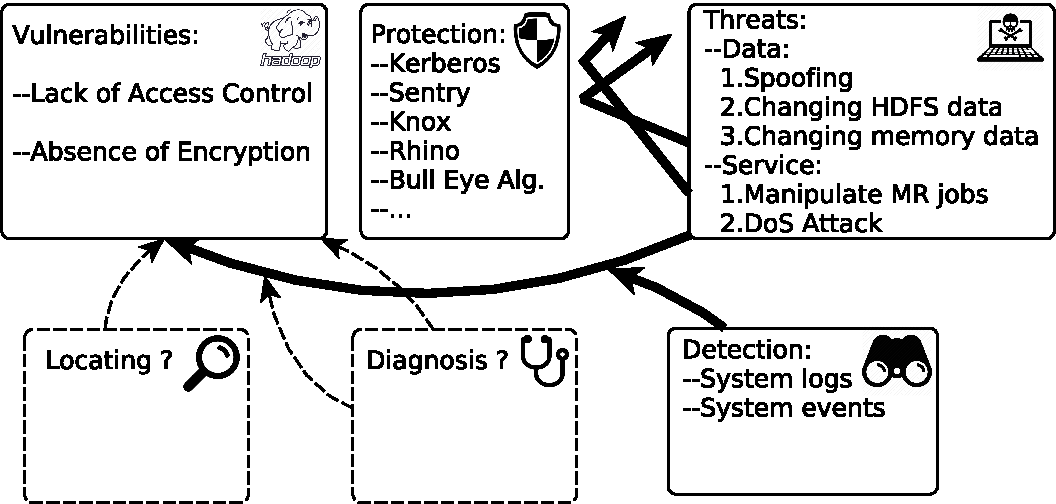
\includegraphics[width=\linewidth]{fig/HadoopSecurity}
			\caption{Security Issues of Hadoop Clusters}
			\label{fig:hadoop-security}
		\end{figure}

		\begin{figure}[!t]
			\centering
			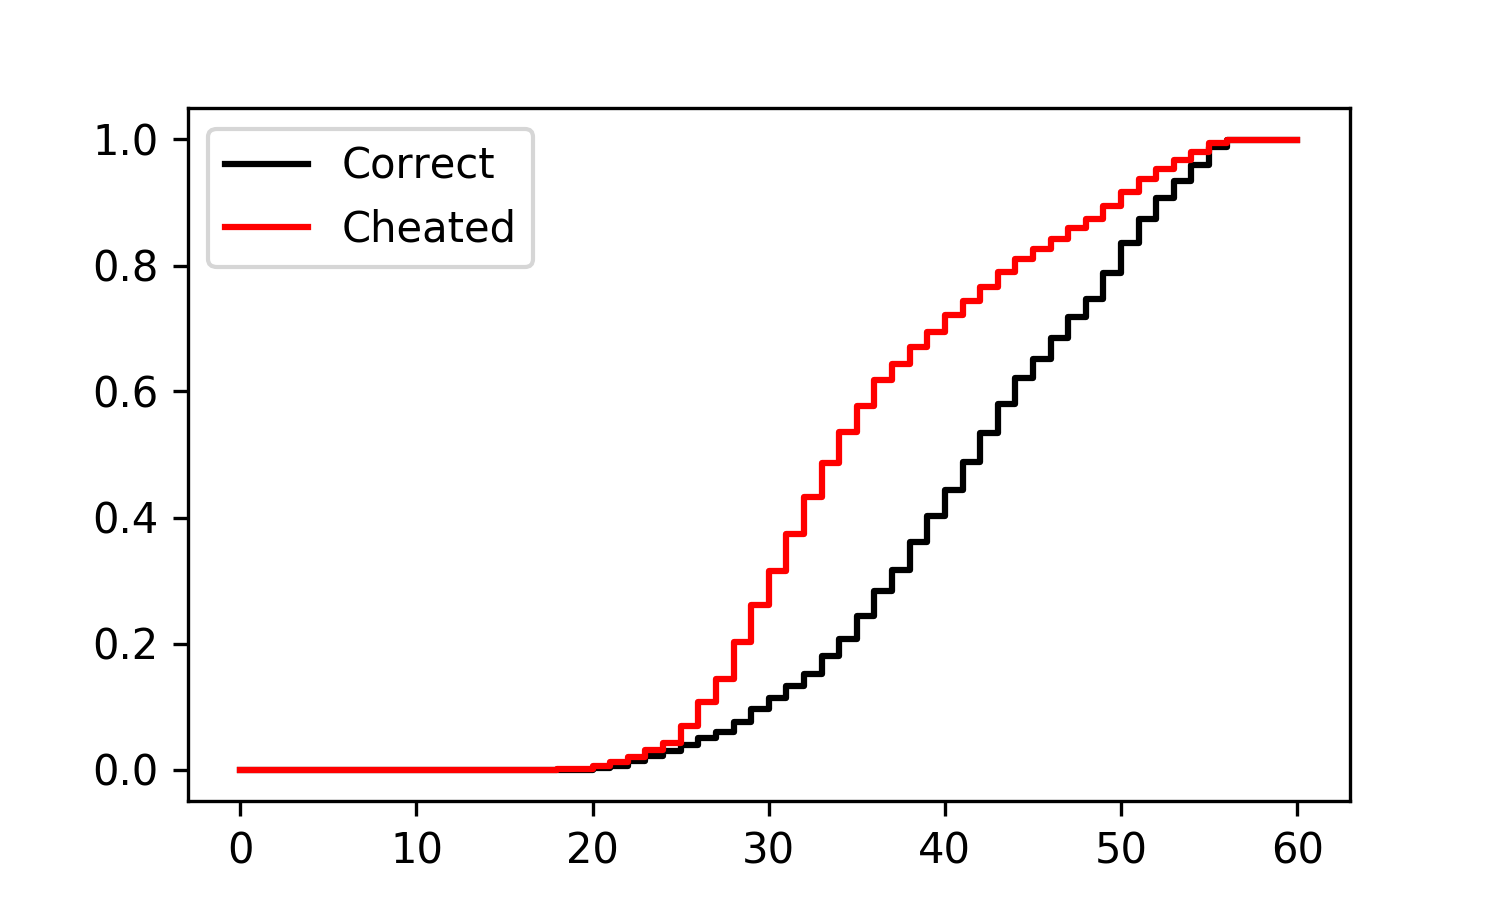
\includegraphics[width=\linewidth]{fig/ExampleEcdf.png}
			\caption{Example Cumulative Distribution Function of Original And Modified Data}
			\label{fig:example-ecdf}
		\end{figure}
		
		According to our observation, typical data manipulations on numerical data will lead to the drift of its distribution. For example, a Taobao online seller's transaction records can be ``click farmed'' to increase the volume of sales. Fig.~\ref{fig:example-ecdf} shows the sales distribution within one day. The curve for cheated data is emulated according to a popular method for click farming. It can be observed that there exists clearly a gap between these two distributions. 		
		%For example, in a sampled data set from Melbourne city pedestrian volume along main streets\footnote{https://data.melbourne.vic.gov.au/Transport-Movement/Pedestrian-volume-updated-monthly-/b2ak-trbp}, 20\% records were randomly selected and modified, the value set as a tenth of the original. The empirical cumulative distribution function of the two data sets are shown in Fig.~\ref{fig:example}, where there is clearly a gap between these distributions.
		These anomalies inside data pipelines will severely affect mining and learning algorithms and further change the final decision given by the entire system.
		
		In order to address issues resulted from data manipulation and pipeline errors, we propose a novel mechanism to detect and locate corrupted data within a data pipeline via statistical distance. As far as we know, this algorithm is the first attempt against data anomaly via statistical distance. Evaluations are performed on synthetic and real-world data sets, demonstrating the correctness and effectiveness of the mechanism.
		
		The rest of the paper is organised as follow: Section~\ref{sec:related-work} introduces preliminaries and recent works on data anomaly detection and statistical distance. Algorithm details are proposed in section~\ref{sec:algorithm-details}. Section~\ref{sec:evaluation} presents evaluation results and further findings of the algorithm. And all contents are concluded in section~\ref{sec:conclusion}.
	
	\section{Preliminaries and Related Work}\label{sec:related-work}
		\subsection{Data Anomaly Detection}
			Anomaly detection, also known as outlier detection, has been studied for a long time and discussed in diverse research domains, such as fraud detection, intrusion detection, system monitoring, fault detection and event detection in sensor networks. According to a systematic classification in~\cite{chandola2009anomaly}, anomaly detection algorithms deal with input data in the form of points(or records), sequences, graphs and spatial relationships, where point data is the simplest and well studied, others are attracting more attention in new studies.
			
			Prevalent anomalies can be classified into \textit{Point Anomalies}, \textit{Contextual(or Conditional) Anomalies} and \textit{Collective Anomalies}. Point anomalies refers to an individual data instance that is considered anomalous with respect to others. But if it is anomalous only in certain circumstances or a specific context, the instance is regarded as contextual anomaly. If a group of related data(e.g. a segment of sequence) instances is anomalous with respect to other groups in the data set(e.g. the entire sequence), it is called a collective anomaly.
			
			Detection approaches can be categorized into three types according to whether data is labeled: \textit{Supervised}, \textit{Semi-Supervised} and \textit{Unsupervised} anomaly detection. As the name suggests, supervised detection methods train models on completely labeled data while unsupervised detection leverages data without any labeling. Semi-supervised detection approaches train model on data that has labeled instances for only the normal class. Supervised detection is commonly applied when both normal and anomalous data can be obtained. When it comes to the circumstances that anomalous data is hard to obtain or there exist too many diverse types of anomalies to enumerate, semi-supervised or unsupervised approaches are usually taken into consideration.
			
			To make the final decision, detection algorithms mostly yield a score from each input instance, denoting how likely it is anomalous. The algorithm then selects top few as anomalies or compare the score with a threshold. Or, detection algorithms output a label on each instance, then decide whether each label belongs to the normal class.
			
			Currently, distance based~\cite{cao2014scalable,cao2017multi} and feature evolving algorithms~\cite{masud2013classification,li2015discovery,shao2014prototype} algorithms seize most attention. Others adopted tree isolation~\cite{zhang2017lshiforest}, model based~\cite{yin2016model} and statistical methods~\cite{zhu2002statstream} in certain applications.
			
			To detect collective anomalies,~\cite{caudell1993adaptive} adopted the \textit{ART(Adoptive Resonance Theory)} neural networks to detect time-series anomalies. \textit{Box Modeling} is proposed in ~\cite{chan2005modeling}. And \textit{Longest Common Subsequence} was leveraged in ~\cite{budalakoti2006anomaly} as similarity metric for symbolic sequence. Markovian modeling techniques are also popular in this domain\cite{ye2000markov,warrender1999detecting,pavlov2003sequence}. \cite{yu2015glad} depicted groups in social media as combinations of different ``roles'' and compare groups according to the proportion of each role within each group.
		
		\subsection{Click Farming Detection}
		
		\subsection{Statistical Divergence}
			Statistical divergence, also called statistical distance, is a function which describes the ``distance'' of one probability distribution to the other on a statistical manifold. Suppose $S$ is a space of probability distributions, then a divergence is a function from $S$ to non-negative real numbers: 
			\begin{equation}
				D(\cdot || \cdot): S \times S \rightarrow \mathbb{R^+}
			\end{equation}
			
			Divergence between two distributions $P$ and $Q$, written as $D(P||Q)$, satisfies:
			
			\begin{enumerate}
				\item $D(P||Q) \ge 0, \forall P, Q \in S$
				\item $D(P||Q) = 0$, if and only if $P=Q$
			\end{enumerate}
			
			There are many ways to calculate divergence, such as f-divergences, M-divergences and S-divergences. Some of them provides better properties which brings conveniences to the design and implementation of our approach.
			
			\subsubsection{Kullback-Leibler Divergence}
			$P,Q$ are discrete probability distributions, $Q(i)=0$ implies $P(i)=0$ for $\forall i$, the \textit{Kullback-Leibler Divergence} from $Q$ to $P$ is defined to be:
			
			\begin{equation}
			KLD(P||Q) = \sum_{Q(i)\ne 0} P(i)log\Big(\frac{P(i)}{Q(i)}\Big)
			\end{equation}
			
			\subsubsection{Jensen-Shannon Divergence}
			$P,Q$ are discrete probability distributions, \textit{Jensen-Shannon Divergence} between $P$ and $Q$ is defined to be:
			
			\begin{equation}
			JSD(P||Q) = \frac{1}{2}KLD(P||M) + \frac{1}{2}KLD(Q||M)
			\end{equation}
			where $\displaystyle M = \frac{1}{2}(P+Q)$.
			
			A more generalized form is defined to be:
			
			\begin{equation}
			JSD_{\pi_1, \dots, \pi_n}(P_1, \dots, P_n) = \sum_{i=1}^{n}\frac{1}{\pi_i}KLD(P_i||M)
			\end{equation}
			where $\displaystyle M = \sum_{i=1}^{n}\frac{1}{\pi_i}P_i$ and $\displaystyle \sum_{i=1}^{n}\frac{1}{\pi_i} = 1$.
			
			Jensen-Shannon divergence has some fine properties:
			\begin{enumerate}
				\item $JSD(P||Q) = JSD(Q||P), \forall P, Q\in S$.
				\item $0 \le JSD_{\pi_1, \dots, \pi_n}(P_1, \dots, P_n) \le log_k(n)$. If a $k$ based algorithm is adopted.
				\item To calculate $JSD(P||Q)$, it need not necessarily to be true that $Q(i)=0$ implies $P(i)=0$.
			\end{enumerate}
		
			\textbf{[If P, Q are continuous distribution?]}
	
	\section{Algorithm Details}\label{sec:algorithm-details}
		Diverse data sets in the real world show certain structures which may be resulted from hidden patterns or relationships among records in a collection of data. For example, the volume of vehicles in the highway and the business transaction records, they may show a relatively stable distribution in the daily scale. Manipulation on those data(e.g. Fig~\ref{fig:example-ecdf}) results in a drift or distortion of the distribution, which can be captured to trigger the alarm.
		Although the population parameters(e.g. mean, variance, etc.) are unknown and usually impossible to obtain, it can be sampled and estimated according to the central limitation theorem.
		
		\subsection{Technical Points}
			\textbf{[Can be divided and settled inside later two subsections]}
			\begin{enumerate}
				\item Which classifier should be chosen?
				\item How to determine the classifier threshold?\textbf{[fixed value, 3$\sigma$]}
				\item How to locate the compromised component?
				\item How to deal with slightly drifting distribution?
				\item .[to be continued \dots]
			\end{enumerate}
			
		\subsection{Divergence-Based Collective Anomaly Detection}
			Suppose data chunks in the given data set $S$ are groups of instances sampled from a population driven by a static distribution. And we are given in advance an evidence set $E$ which contains $n(n\ge2)$ collections of correct sample data. Then each data collection in $S$ can be checked by the following algorithm.
			
			\begin{algorithm}[!ht]
				\caption{Basic Classification}
				\label{alg:static}
				\begin{algorithmic}[1]
					\Require Evidence set $E = \{D_1, \dots, D_n\}$; New data collection $D'$
					\Ensure Whether $D'$ is anomalous
					\For{$i \gets 1$ to $n$ do}
						\State $P_i \gets$ the distribution of $D_i$
					\EndFor
					\State $M \gets \frac{1}{n}\sum_{i=1}^{n}P_i$\label{line:population-estimation}
					\For{$i \gets 1$ to $n$ do}
						\State $J_i \gets JSD(P_i||M)$
					\EndFor
					\State $N \gets$ normal distribution estimated from $J_1, \dots, J_n$
					\State $P' \gets$ distribution of $D'$
					\State $J' \gets JSD(P'||M)$
					\State $p \gets$ probability density of $J'$ in $N$
					\If{$p <$ threshold $T$}
						\State \textbf{Return} True
					\Else
						\State \textbf{Return} False
					\EndIf
				\end{algorithmic}
			\end{algorithm}
		
			As shown in Algorithm~\ref{alg:static}, $n$ evidence collections are used to estimate the ground truth population distribution $M$. Then $n$ evidence divergences are calculated, composing a gaussian classifier to classify the new distribution sample. Although it is convenient to compute $JSD(P_1, \dots, P_n, P')$ instead of $JSD(P_1||M), \dots, JSD(P_n||M), JSD(P'||M)$. It is not suitable for classification. Jensen-Shannon divergence of $n+1$ distributions will dilute the affection of the abnormal one, in which case the difference between $P'$ being normal and anomalous will become subtle when $n$ goes larger.
			
			Similar to the fact that sampling values around a certain parameter will yield a gaussian distribution, sampling divergences around a certain population distribution yields a gaussian distribution $N(\mu, \sigma)$ where $\mu$ is a value slightly larger than zero. $\mu$ can not be zero according to line~\ref{line:population-estimation}. $M$ takes into consideration all existing values in every distribution sample and averages corresponding probabilities. Thus $M$ may consist entries that does not exist in $P_i$ and probability in certain entries in $M$ may vary from that in $P_i$. For example, suppose $P_1(1)=0.5, P_1(2)=0.3, P_1(3)=0.2$; $P_2(1) = 0.3, P_2(2) = 0.4, P_2(3) = 0.3$; $P_3(1)=0.3, P_3(3)=0.5, P_3(4)=0.2$, then $M(1) = \frac{11}{3}, M(2)=\frac{7}{3}, M(3)=\frac{10}{3}, M(4)=\frac{2}{3}$. None of $P_1, P_2, P_3$ is the same with $M$. Although the distance cannot be negative values, normal distribution is the closest to the distribution of all JSD values.
		
		\subsection{Distribution Histogram}\label{sec:alg-histogram}
			Not all data collections can be assumed subject to known distribution models. Parameter approximation will probably lead to errors above our expectation. For example, the distribution of vehicle volume in the highway may not correspond to any of the prevalent distribution model. Few assumption of parameters can be made in advance on such data. For the sake of generality, non-parametric estimation should be applied.
			
			Surely, the kernel density estimation approaches will give a smooth, continuous distribution curve under on any sampled data. The computational cost will be much higher than applying a coarse histogram approximation.
			Moreover, even if we applied a distribution model upon a collection of sampled data, yielding more accurate results, the computation of divergence will be much more complex on continuous functions than discrete distributions.
			
			Histogram methods can not only be applied to non-parametric distributions, but also to miscellaneous data types. From a general point of view, as long as there exits a function mapping the input data instance into a subset of real numbers, this data collection can be counted into a histogram. For example, date, time and single characters.
			
			In order to generate a accurate approximation, step size is the most important parameter the algorithm should determine. If the size is too small then the resulting histogram will be over fitting; but if the size is too large then the estimation will be too coarse to depict the original shape. According to statistics theory, when dealing with a sample size of $k$, a step size of 
			
			\begin{equation}\label{equ:step-size}
				l = c \sigma k^{-0.2}
			\end{equation}
			
			will give a best partition, where $c$ is a constant relative to the shape of distribution(e.g. for normal distribution, $c=1.05$).
			
		\subsection{Threshold}\label{sec:alg-threshold}
			One important factor in the algorithm is the value of threshold. A higher threshold rejects more instances, improving the sensitivity of anomalous data while increasing the number of false alarms. A lower threshold provide higher true negative rates yet neglecting more possible threats.
			
			A naive but prevalent approach is to set a fixed value as threshold. This approach is easy to implement and may give satisfying results in specific cases. However, a fixed threshold requires analysis of the specific problem, manual observation and tuning of parameters, which involves lots of human labor. The rule of ``$3 \sigma$'' can be used to automatically determine a threshold. But in some cases that the anomalous data intersecting at the boundary with normal instances, the threshold may fail more often to discover those manipulated ones.
			
			However, applying divergence as the distance metric among data collection distributions provides a fine property. That is, divergences of normal data collections assemble together, forming a quasi-normal distribution. And those of anomalous data collections lies in the right-hand-side interval on the real number axis. As a result of further observation, the divergence of anomalous data collections also assemble to be a quasi-normal distribution, since statistical distance has been restricted by a strict upper bound.
			
			\textbf{[Better give a point drawing for each JSD value]}
			
			\begin{figure}[!ht]
				\centering
				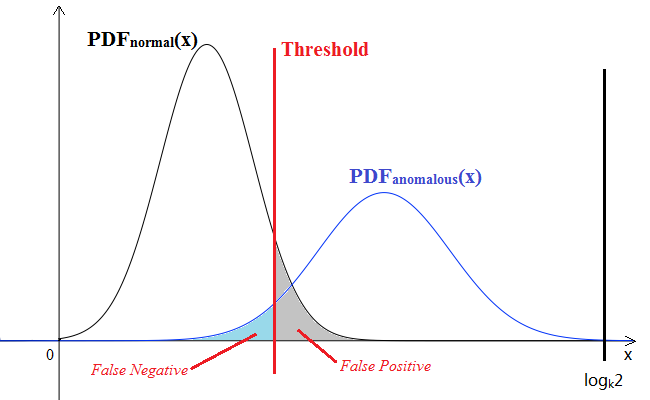
\includegraphics[width=\linewidth]{fig/ExampleThreshold.png}
				\caption{Threshold Example}
				\label{fig:example-threshold}
			\end{figure}
			
			As shown in Fig~\ref{fig:example-threshold}, the black curve($PDF_{normal}(x)$) displays the probability density function(PDF) fitting those JSDs calculated from normal data collections; the blue curve($PDF_{anomalous}(x)$) displays the PDF derived from anomalous data collections. Threshold is to minimize total error(False Negative and False Positive).
			
			Suppose:
			
			\begin{align}
				PDF_{normal}(x) &\approx N(\mu_n, \sigma_n)\\
				PDF_{anomalous}(x) &\approx N(\mu_a, \sigma_a)
			\end{align}
			
			Then the optimal threshold $T$ is:
			
			\begin{equation}\label{equ:linear-weight}
				\small
				\begin{split}
					T &= \mathop{\arg\min}_{T} \int_{0}^{T}PDF_{anomalous}(x)dx +
					 \int_{T}^{log_k2}PDF_{normal}(x)dx\\
					& \approx \mathop{\arg\min}_{T}
					\int_{-\infty}^{T}
					\frac{e^{-\frac{(x - \mu_a)^2}{2\sigma_a^2}}}{\sqrt{2\pi} \sigma_a}dx
					+ \int_{T}^{+\infty}
					\frac{e^{-\frac{(x - \mu_n)^2}{2\sigma_n^2}}}{\sqrt{2\pi} \sigma_n}dx\\
					& = \frac{\mu_n\sigma_a + \mu_a\sigma_n}{\sigma_a + \sigma_n}
				\end{split}
			\end{equation}
			
			According to equation(\ref{equ:linear-weight}), threshold value can be automatically determined. The optimal threshold will minimize total errors, yielding an optimal outcome. The only requirement for this technique is another evidence set containing data point derived from anomalous data collections.
			
			However, this is not accurate enough, since equation(\ref{equ:linear-weight}) implicate an assumption that the chances are the same for a new data collection to be either anomalous or not. If we can determine the probability for a new data collection to be anomalous in any segment of data sequence, the equation should be modified as:
			
			\begin{equation}\label{equ:linear-balanced}
				\small
				\begin{split}
					T & = \mathop{\arg\min}_{T} \alpha\int_{0}^{T}PDF_{anomalous}(x)dx +
				(1-\alpha)\int_{T}^{log_k2}PDF_{normal}(x)dx\\
					& \approx \mathop{\arg\min}_{T}
					\alpha\int_{-\infty}^{T}
					\frac{e^{-\frac{(x - \mu_a)^2}{2\sigma_a^2}}}{\sqrt{2\pi} \sigma_a}dx
					+ (1-\alpha)\int_{T}^{+\infty}
					\frac{e^{-\frac{(x - \mu_n)^2}{2\sigma_n^2}}}{\sqrt{2\pi} \sigma_n}dx
				\end{split}
			\end{equation}
			
			Where $\alpha$ is the anomaly probability. Equation(\ref{equ:linear-balanced}) is much more complicated than (\ref{equ:linear-weight}). It can be reduced to a quadratic equation. But may not have real roots in all cases.
			
			From another point of view, equation (\ref{equ:linear-weight}) can be regarded as a weighted averaging between two mean value: $\mu_n$ and $\mu_a$. From this aspect, we can derive some similar approximations:
			
			\begin{align}
				T &= \frac{\mu_n \sqrt{\sigma_a} + \mu_a \sqrt{\sigma_n}}{\sqrt{\sigma_a} + \sqrt{\sigma_n}}
				\label{equ:sqrt-weight}\\
				T &= \frac{\mu_n \sigma_a \sqrt{-ln(1 - \alpha)}
					+ \mu_a \sigma_n \sqrt{-ln\alpha}}
				{\sigma_a \sqrt{-ln(1 - \alpha)} + \sigma_n \sqrt{-ln\alpha}}
				\label{equ:sqrt-log-add-weight}\\
				T &= \frac{\mu_n \sqrt{|ln\big[\sigma_a (1 - \alpha)\big]|}
					+ \mu_a \sqrt{|ln(\sigma_n \alpha)|}}
				{\sqrt{|ln\big[\sigma_a (1 - \alpha)\big]|} + \sqrt{|ln(\sigma_n \alpha)|}}
				\label{equ:sqrt-log-combined-weight}
			\end{align}
			
			Due to the restriction sample capacity, the replacement of JSD distributions by guassian distribution may lose too much accuracy. Compared with equation (\ref{equ:sqrt-weight}), (\ref{equ:sqrt-log-add-weight})and (\ref{equ:sqrt-log-combined-weight}), (\ref{equ:linear-balanced}) may not give a best result.
		
		\subsection{Dynamic DCAD}
			Another important factor that should be seriously considered is the assumption in Algorithm~\ref{alg:static}. In most cases, real world data is always in the process of evolution and fluctuation. Therefore, the algorithms should automatically adapt to the trend at any time. To meet the need, a sliding window technique has been applied to the basic algorithm frame work. Considering discussion in section~\ref{sec:alg-histogram} and~\ref{sec:alg-threshold}, a dynamic version is proposed as follow:
			
			\begin{algorithm}[!ht]
				\caption{Dynamic DAD}
				\label{alg:dynamic}
				\begin{algorithmic}[1]
					\Require Normal evidence set $E_N = \{D_{N_1}, \dots, D_{N_n}\}$ by given order; Anomalous evidence set $E_A = \{D_{A_1}, \dots, D_{A_m}\}$ by given order; New data collection $D'$; Estimated anomalous probability $\alpha$
					\Ensure Whether $D'$ is anomalous
					\For{$i \gets 1$ to $n$}
						\State $P_{N_i} \gets$ histogram of $D_{N_i}$
					\EndFor
					\For{$i \gets 1$ to $m$}
						\State $P_{A_i} \gets$ histogram of $D_{A_i}$
					\EndFor
					\State $P' \gets$ histogram of $D'$
					\State $M \gets \frac{1}{n}\sum_{i=1}^{n}P_{N_i}$
					\For{$i \gets 1$ to $n$}
						\State $J_{N_i} \gets JSD(P_{N_i}||M)$
					\EndFor
					\For{$i \gets 1$ to $m$}
						\State $J_{A_i} \gets JSD(P_{A_i}||M)$
					\EndFor
					\State $J' = JSD(P'|||M)$
					\State $(\mu_N, \sigma_N) \gets$ estimated from $\{J_{N_1}, \dots, J_{N_n}\}$
					\State $(\mu_A, \sigma_A) \gets$ estimated from $\{J_{A_1}, \dots, J_{A_m}\}$
					\State $T \gets$ proper threshold derived from $(\mu_N, \sigma_N)$, $(\mu_A, \sigma_A)$ and $\alpha$
					\If{$J' < T$}
						\State $E_N \gets E_N \backslash \{D_{N_0}\} \cup \{D'\}$\label{line:update-normal-evidence}
						\State \textbf{Return} False
					\Else
						\State $E_A \gets E_A \backslash \{D_{A_0}\} \cup \{D'\}$\label{line:update-anomalous-evidence}
						\State \textbf{Return} True
					\EndIf
				\end{algorithmic}
			\end{algorithm}
			
			Algorithm~\ref{alg:dynamic} uses $E_N$ and $E_A$ as two sliding windows, keeping up with latest trend of both normal and anomalous features. Thus, the two window sizes $n$ and $m$ cannot be too large. Otherwise the evolving features will be flattened and aligned to the older ones. For the sake of estimation accuracy, they cannot be too small either. The size should refer to ratio of both data updates and feature evolution.
			
			Line~\ref{line:update-normal-evidence} and~\ref{line:update-anomalous-evidence} update the evidence sets, replacing the most outdated one, moving the sliding window forward one step ahead. Moreover, $\alpha$ can also be updated according to a history sequence of return values, if necessary.
	
	\section{Evaluation}\label{sec:evaluation}
		\subsection{Experiment Environment}
			The algorithm was implemented and interpreted in Python 3.6. All experiments was tested on Ubuntu 17.04.
		
		\subsection{Methodology}
			\textbf{Raise and answer some research questions. Present test background and methods.}
			
			We adopted a data set containing Taobao online sellers' transaction records\footcite{https://tianchi.aliyun.com/competition/information.htm?raceId=231591} provided by Alibaba Tian Chi big data competition. The data package contains seller features data set, user payments data set and user browsing behaviour data set. An example of the user payments data set is shown in Table~\ref{tab:user-payment-sample}.
			
			\begin{table}[!ht]
				\centering
				\caption{User Payment Record Exmaple}
				\label{tab:user-payment-sample}
				\begin{tabular}{|c|c|c|}
					\hline
					User ID & Seller ID & Payment Time\\
					\hline
					10523185 & 1629 & 2015-11-11 17:00:00\\
					\hline
					2 & 2 & 2\\
					\hline
					3 & 3 & 3\\
					\hline
					\vdots & \vdots & \vdots\\
					\hline
				\end{tabular}
			\end{table}
			
			We randomly chose one seller(ID: 1629) and extracted transaction history of this seller, records ranging from Nov. 11th 2015 to Oct. 31st 2016. Entire transaction set was then divided into 325 collections, each containing records in one day. 
			
			
			\begin{figure}[!ht]
				\centering
				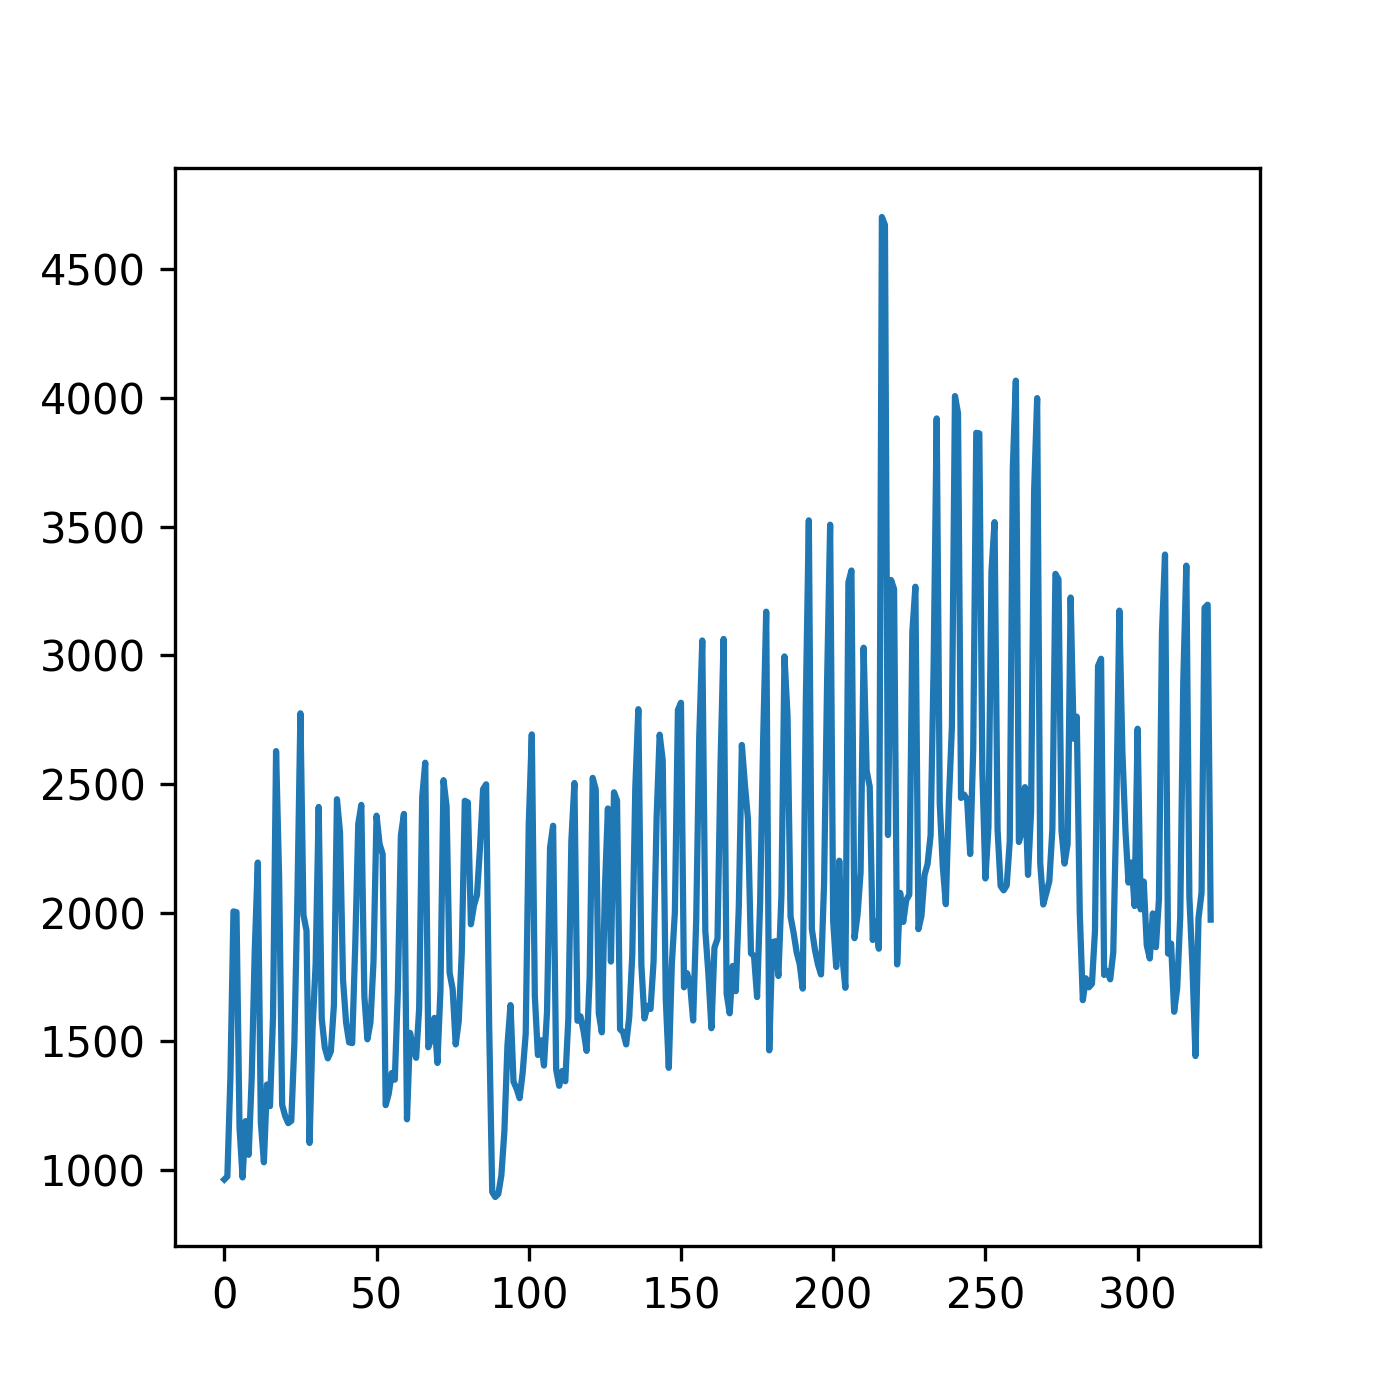
\includegraphics[width=0.75\linewidth]{fig/DailyTransactionVolume.png}
				\caption{Daily Transaction Volumes}
				\label{fig:daily-transaction-volume}
			\end{figure}
			
			\begin{figure}[ht]
				\centering
				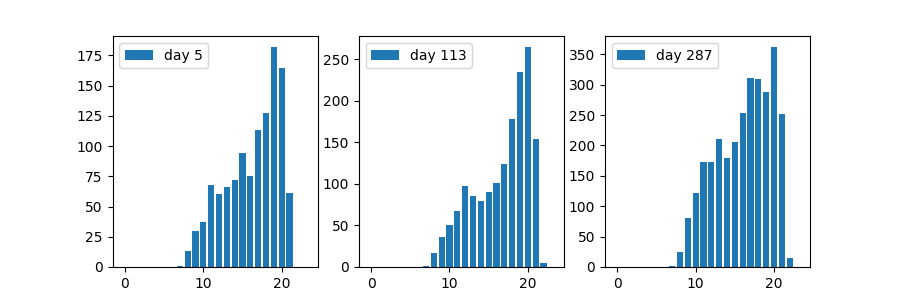
\includegraphics[width=\linewidth]{fig/SaleDistributionSamples.png}
				\caption{Randomly selected 3 days and draw histograms by hourly sale}
				\label{fig:sale-distribution-sample}
			\end{figure}
			
			Fig.~\ref{fig:daily-transaction-volume} shows the daily transaction volume of the seller. It sees a trend of daily sale which is slightly moving as the time goes. And the daily selling distributions, as is shown in Fig.~\ref{fig:sale-distribution-sample}, display a roughly similar shape.
			
			Click farmed data was generated according to patterns described in online reports\textbf{[ref here]}. The most popular way of click farming is to call online a group of people, assign each of them an amount of transaction. And those ``employees'' individually buy certain products via different buyer accounts. Therefore, a significant feature of this approach is that the cheating transactions usually assemble together in a short period of time. It is called ``Centralized Farming''. Some other ``employers'' are more clever. They usually arrange a time table for each employee to create new transactions. Thus the transaction distribution may not vary too much with and without click farming. This is called ``Equalized Farming''.
			
			To emulate ``Centralized Click Farming'', we randomly inserted some gaussian-distributed transactions in a chosen collection, where the total number of new records is the same of the original volume. To emulate a extremely clever ``Equalized Click Farmer'', we simply doubled each record in the chosen collection to make the new distribution exactly the same as the original one, which is harder for the online platform to discover.
			
			To play the role of purchasing platform, we surveillance two levels of transaction distribution. The first level is simply drawing a histogram on time spans. The second level is to draw a histogram on the sub-volumes of each time span. For example, shown in Fig.~\ref{fig:histogram-example}, the first level histogram can be drawn by counting the number of hourly sales. The frequencies of each bucket in 1st level histogram is: $F=$\{0, 0, 0, 0, 0, 0, 0, 1, 13, 30, 37, 68, 60, 66, 72, 94, 75, 113, 127, 182, 165, 61, 0, 0\}. Then, counting $F$ with a step size 20 gives the 2nd level histogram.
			
			\begin{figure}[!ht]
				\centering
				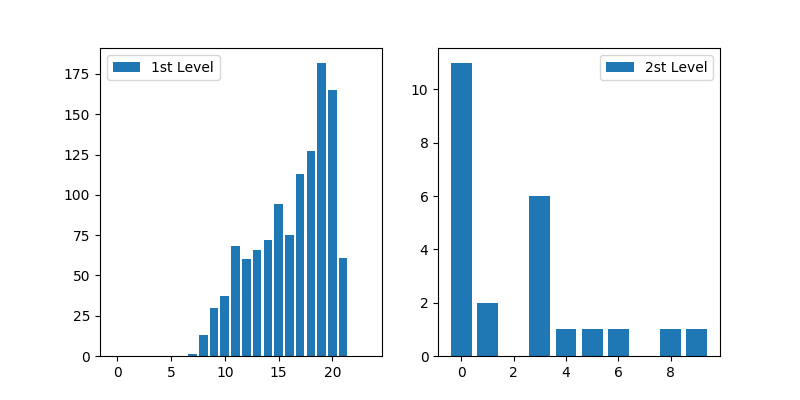
\includegraphics[width=\linewidth]{fig/HistogramExample.png}
				\caption{Example of 1st and 2nd Level Histogram}
				\label{fig:histogram-example}
			\end{figure}
			
			In order to test the performance of Algorithm~\ref{alg:dynamic}, every single collection was fed into the algorithm by the time order. Each collection input has a probability of $\alpha$ to be anomalous, namely, click farmed. The algorithm checks each collection with 1st or 2nd level histogram and give an answer of true and false. Then a F1 score was computed as the result of the experiment.
			
		\subsection{Experiment on Raw Data}
			We first tested Algorithm~\ref{alg:dynamic} on raw data set in order to see whether and why the algorithm works. Due to desensitization process, time stamps in raw data set only tell which hour the transaction was committed. Thus, the histogram was drawn by counting hourly volume of each collection. For $\alpha = 0.2$, we select first 30 days as the evidence set of normal collections; day 21st to 30th were also emulated to be click farmed, composing the evidence set of anomalous collections. Equation(\ref{equ:sqrt-log-add-weight}) was employed as the threshold calculator. The results are shown in Table~\ref{tab:result-raw-1st}, where \textit{true positive rate}, \textit{false positive rate} and \textit{accuracy} were recorded.
			
			\begin{table}[!ht]
				\centering
				\caption{Classification Results on Raw Data}
				\label{tab:result-raw-1st}
				\begin{tabular}{|c|c|c|c|c|c|c|}
					\hline
					& \multicolumn{3}{c|}{Centralized} & \multicolumn{3}{c|}{Equalized}\\
					\hline
					& TPR & FAR & ACC & TPR & FAR & ACC\\
					\hline
					1st Level & 100 & 4.05 & 96.72 & 26.64 & 28.03 & 62.49\\
					\hline
					2nd Level & 88.01 & 7.68 & 91.41 & 83.89 & 15.78 & 84.07\\
					\hline
				\end{tabular}
			\end{table}
			
			\begin{figure}[!ht]
				\centering
				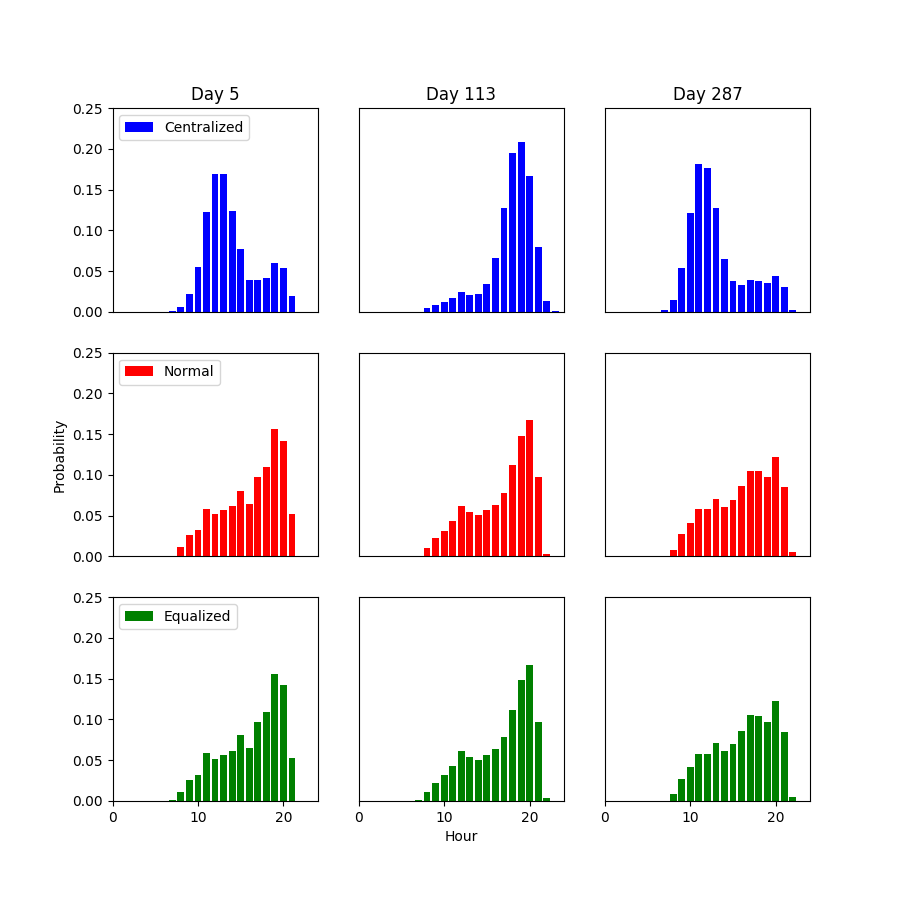
\includegraphics[width=\linewidth]{fig/Raw1stLevelHist.png}
				\caption{1st Level Histogram of Raw Data}
				\label{fig:raw-hist-1st}
			\end{figure}
			
			\begin{figure}[!ht]
				\centering
				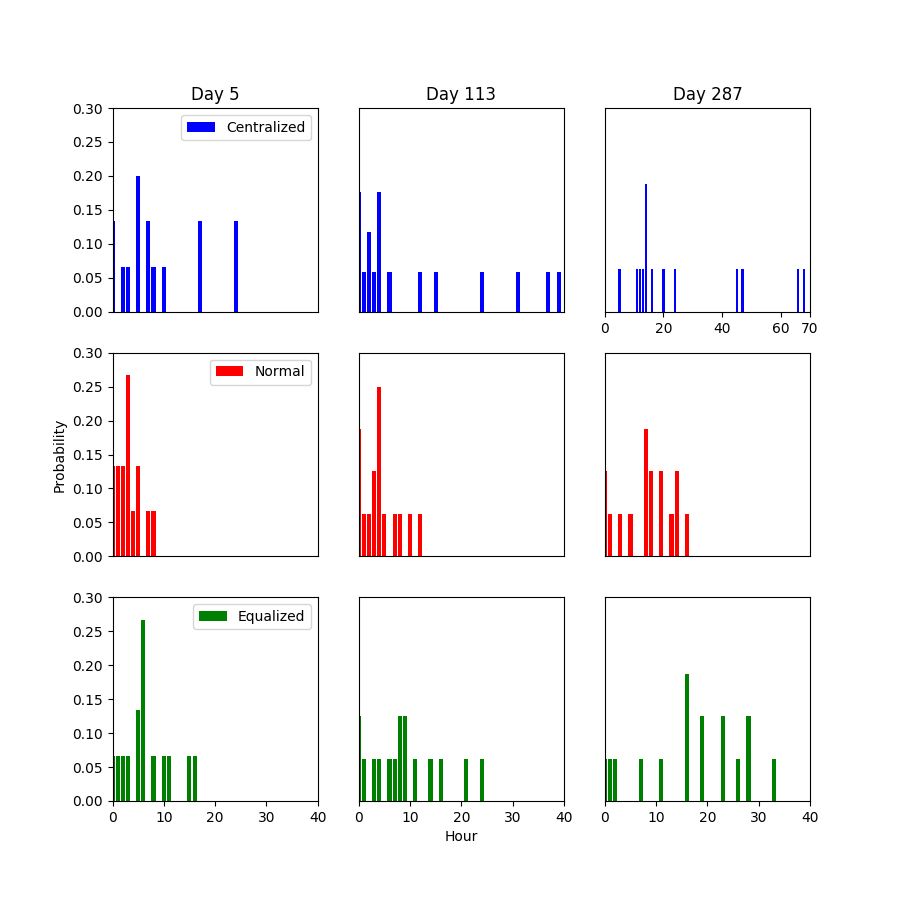
\includegraphics[width=\linewidth]{fig/Raw2ndLevelHist}
				\caption{2nd Level Histogram of Raw Data}
				\label{fig:raw-hist-2nd}
			\end{figure}
			
			\begin{figure}[!ht]
				\centering
				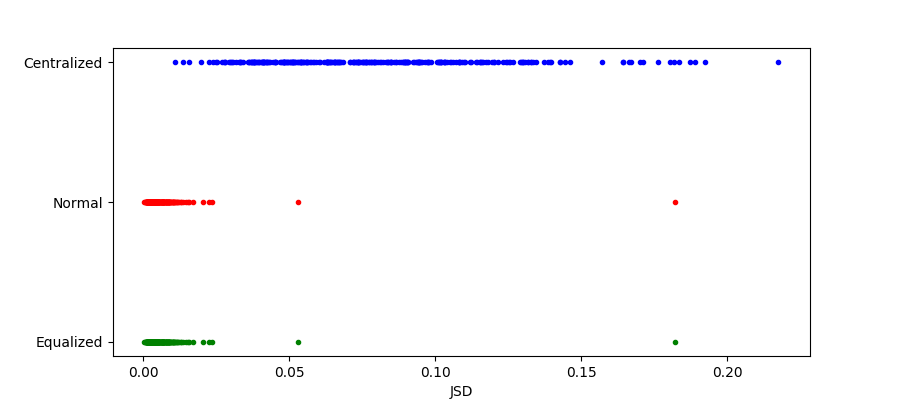
\includegraphics[width=\linewidth]{fig/RawOverview1st.png}
				\caption{JSD of 1st Level Histograms}
				\label{fig:raw-overview-1st}
			\end{figure}
			
			\begin{figure}[!ht]
				\centering
				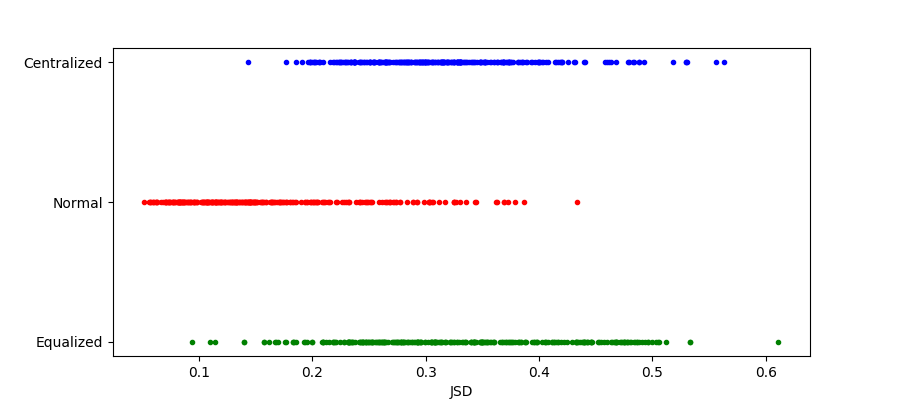
\includegraphics[width=\linewidth]{fig/RawOverview2nd.png}
				\caption{JSD of 2nd Level Histogram}
				\label{fig:raw-overview-2nd}
			\end{figure}
			
			When classifying toward 1st level histograms, centralized click farming behaviours can be easily discovered. As displayed in the left two columns in Fig.~\ref{fig:raw-hist-1st}, normal collections share a similar distribution while centralized click farmed ones abruptly violates the original shape. However, as a clever click farmer, equalized click farming did not in the least distorted the distribution. Most of them escaped the security check under the perfect disguise.
			But when it comes to 2nd level histogram, the ``clever disguise'' does not work any longer. It can be clearly seen in Fig.~\ref{fig:raw-hist-2nd} that both types of click farming shows an obvious difference from the normal ones, while the normal ones still share a similar distribution.
			From the overview in Fig.~\ref{fig:raw-overview-1st} and~\ref{fig:raw-overview-2nd}, the difference between normal and anomalous collections can be observed more intuitively.
			
		\subsection{Experiment on Synthetic Data}
			As is put in the former section, every single record in the transaction set only gives a time stamp aligned at hours. Part of the information was erased with the absence of minutes and seconds. In the following experiments, Every time stamp was assigned a random value for minutes and seconds. Therefore, the synthetic data set should be closer to the real world case. Moreover, the step size in the histograms can now be calculated more precisely. In the 1st level histogram, the constant $c$ in equation(\ref{equ:step-size}) was set to 0.5 since the PDF of daily distribution was approximately a linear function. And in the 2nd level histogram, sub-volumes of every 300 seconds were counted, producing more data points in the 2nd level data collections. Then, constant $c$ in equation(\ref{equ:step-size}) was also set to 0.5 given that the 2nd level histogram was also approximately a linear function.
			We tested algorithm performance for $\alpha \in \{0.1, 0.3, 0.5, 0.7, 0.9\}$, with $E_N$ and $E_A$ the same configuration as before. Results were shown in Table~\ref{tab:syn-result-1st} and~\ref{tab:syn-result-2nd}.
			
			\begin{table}[!ht]
				\centering
				\caption{1st Level}
				\label{tab:syn-result-1st}
				\begin{tabular}{|c|c|c|c|c|c|c|}
					\hline
					& \multicolumn{3}{c|}{Centralized} & \multicolumn{3}{c|}{Equalized}\\
					\hline
					$\alpha$ & TPR(\%) & FPR(\%) & ACC(\%) & TPR(\%) & FPR(\%) & ACC(\%) \\ 
					\hline
					0.1 & 86.10 & 1.14 & 97.40 & 5.75 & 12.28 & 79.66 \\ 
					\hline
					0.2 & 96.43 & 9.83 & 91.30 & 26.97 & 26.47 & 64.29 \\ 
					\hline
					0.3 & 97.95 & 16.49 & 87.68 & 37.46 & 39.46 & 53.67 \\ 
					\hline
					0.4 & 99.18 & 31.94 & 81.30 & 57.23 & 48.32 & 53.79 \\ 
					\hline
					0.5 & 99.33 & 23.40 & 88.25 & 67.67 & 58.23 & 54.46 \\ 
					\hline
					0.6 & 99.62 & 25.70 & 89.83 & 67.03 & 73.78 & 51.64 \\ 
					\hline
					0.7 & 100.00 & 32.51 & 90.51 & 69.69 & 76.28 & 56.16 \\ 
					\hline
					0.8 & 99.72 & 26.97 & 94.35 & 75.56 & 69.44 & 67.00 \\ 
					\hline
					0.9 & 99.63 & 15.73 & 98.19 & 76.59 & 75.18 & 70.73\\
					\hline
				\end{tabular} 
			\end{table}
			
			\begin{table}[!ht]
				\centering
				\caption{2nd Level}
				\label{tab:syn-result-2nd}
				\begin{tabular}{|c|c|c|c|c|c|c|}
					\hline
					& \multicolumn{3}{c|}{Centralized} & \multicolumn{3}{c|}{Equalized}\\
					\hline
					$\alpha$ & TPR(\%) & FPR(\%) & ACC(\%) & TPR(\%) & FPR(\%) & ACC(\%) \\ 
					\hline
					0.1 & 75.60 & 3.90 & 93.74 & 97.84 & 1.64 & 98..31 \\ 
					\hline
					0.2 & 91.93 & 18.43 & 93.73 & 99.42 & 7.39 & 94.01 \\ 
					\hline
					0.3 & 95.01 & 23.70 & 81.69 & 100.00 & 23.93 & 83.05 \\ 
					\hline
					0.4 & 98.09 & 28.66 & 82.49 & 100.00 & 24.59 & 84.75 \\ 
					\hline
					0.5 & 98.33 & 36.54 & 80.00 & 100.00 & 23.76 & 88.36 \\ 
					\hline
					0.6 & 98.35 & 40.69 & 83.41 & 100.00 & 35.94 & 84.63 \\ 
					\hline
					0.7 & 98.54 & 37.97 & 87.80 & 100.00 & 31.27 & 90.84 \\ 
					\hline
					0.8 & 98.47 & 40.38 & 91.19 & 100.00 & 33.04 & 92.66 \\ 
					\hline
					0.9 & 98.51 & 47.56 & 94.58 & 100.00 & 28.44 & 97.40\\
					\hline
				\end{tabular} 
			\end{table}
			
			The result shows that the algorithm can efficiently distinguish the normal and anomalous data collections. No matter how much proportion of data is anomalous, the algorithm always gives a high accuracy. That is because the adaptive threshold was designed to minimize the number of total errors, which was irrelevant to TPR or FPR. When $\alpha$ was increasing, there were less data collections added into $E_N$. Thus the update of $E_N$ became slower and FPR went higher. On the contrary, TPR became higher as $\alpha$ increased. Moreover, since $|E_N| > |E_A|$, it needs more collection instances for $|E_N|$ then that for $|E_A|$ to keep up to the trend. Therefore, it was faster of FPR to increase than TPR to increase. As a result of that, there were more false alarms emerged and ACC went lower, as $\alpha$ increased from 0.1 to 0.5. After that, however, although FPR was still increasing, total number of normal instances decreased dramatically and those false alarms contributed less to total errors. Therefore, ACC rose up again.
			
			\begin{figure}[!ht]
				\centering
				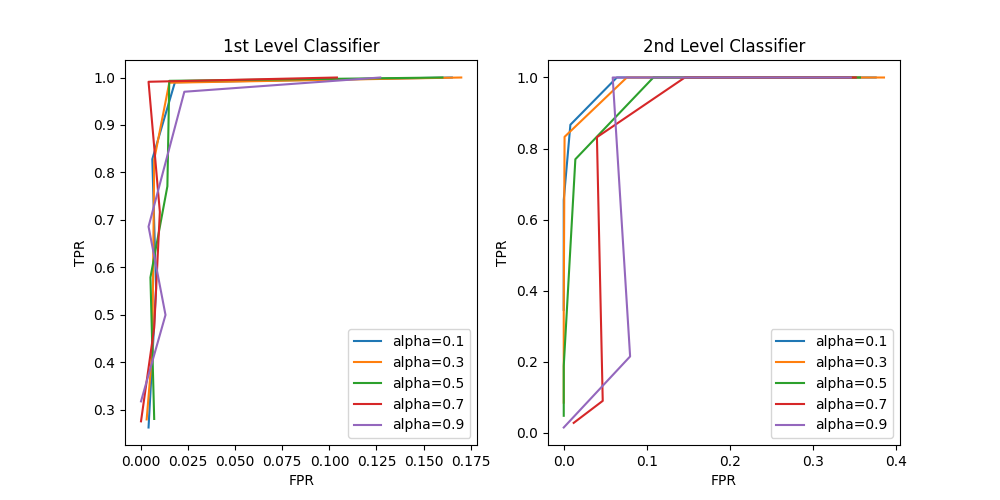
\includegraphics[width=\linewidth]{fig/ROC-alpha}
				\caption{ROC Curve of 1st and 2nd Level Classifier}
				\label{fig:roc-alpha}
			\end{figure}
			
			Fig.~\ref{fig:roc-alpha} shows the ROC curve of the gaussian classifier dealing with centralized click farming with 1st level histogram and equalized click farming with 2nd level histogram.\textbf{[Comment: This shows that the classifier is efficient]}
			
			\begin{figure}[!ht]
				\centering
				This is the figure
				\caption{ROC Curve of Different Magnitude of Click Farming}
				\label{fig:roc-magnitude}
			\end{figure}
			
			\textbf{[Next, show a figure of ROC curve for different click farm magnitude. Explore how sensitive the classifier is for the click farming problem. This requires lots of experiment data. Not finished yet]}
			
		\subsection{Threshold Optimization}
			\textbf{give results of the comparison of different threshold equations, in table~\ref{tab:threshold-comparison}}
			\begin{table*}[!ht]
				\centering
				\caption{Compare of Different Threshold Calculator}
				\label{tab:threshold-comparison}
				\begin{tabular}{|c|c|c|}
					\hline
					Equation & Synthetic & Gaussian \\ 
					\hline
					$T = \frac{\sigma_B \mu_A + \sigma_A \mu_B}{\sigma_B + \sigma_A}$& 1.0588 & 0.5810 \\ 
					\hline
					$T = \frac{\sqrt{\sigma_B} \mu_A + \sqrt{\sigma_A} \mu_B}{\sqrt{\sigma_B} + \sqrt{\sigma_A}}$& 2.1861 & 0.5718 \\ 
					\hline
					$T = \frac{(ln\sigma_B)\mu_A + (ln\sigma_A)\mu_B}{ln\sigma_B + ln\sigma_A}$& 2.2390 & 0.3860 \\ 
					\hline
					$T = \frac{(\sqrt{|ln\sigma_B|})\mu_A + (\sqrt{|ln\sigma_A|})\mu_B}{\sqrt{|ln\sigma_B|} + \sqrt{|ln\sigma_A|}}$& 2.2082 & 0.5515 \\ 
					\hline
					$T = \frac{(ln\sqrt{\sigma_B})\mu_A + (ln\sqrt{\sigma_A})\mu_B}{ln\sqrt{\sigma_B} + ln\sqrt{\sigma_A}}$& 2.1211 & 0.3811 \\ 
					\hline
					$T = \frac{\sigma_B (1 - \alpha) \mu_A + \sigma_A \alpha \mu_B}{\sigma_B (1 - \alpha) + \sigma_A \alpha}$& 0.7688 & 0.3515 \\ 
					\hline
					$T = \frac{(\sigma_B \sqrt{1 - \alpha}) \mu_A + (\sigma_A \sqrt{\alpha}) \mu_B}{\sigma_B \sqrt{1 - \alpha} + \sigma_A \sqrt{\alpha}}$& 0.8158 & 0.4510 \\ 
					\hline
					$
					T = \frac{\big[\sigma_B ln(1 - \alpha)\big] \mu_A
						+ \big[\sigma_A ln\alpha\big] \mu_B}
					{\sigma_B ln(1 - \alpha) + \sigma_A ln\alpha}
					$& 1.5227 & 0.5523 \\ 
					\hline
					$
					T = \frac{\mu_A \sigma_B \sqrt{-ln(1 - \alpha)}
						+ \mu_B \sigma_A \sqrt{-ln\alpha}}
					{\sigma_B \sqrt{-ln(1 - \alpha)} + \sigma_A \sqrt{-ln\alpha}}
					$& 2.6013 & 0.5791 \\ 
					\hline
					$
					T = \frac{\mu_A \sigma_B ln\sqrt{1 - \alpha}
						+ \mu_B \sigma_A ln\sqrt{\alpha}}
					{\sigma_B ln\sqrt{1 - \alpha} + \sigma_A ln\sqrt{\alpha}}
					$& 1.4155 & 0.5578 \\ 
					\hline
					$
					T = \frac{\mu_A \sqrt{|ln\big[\sigma_B (1 - \alpha)\big]|}
						+ \mu_B \sqrt{|ln(\sigma_A \alpha)|}}
					{\sqrt{|ln\big[\sigma_B (1 - \alpha)\big]|} + \sqrt{|ln(\sigma_A \alpha)|}}
					$& 2.2730 & 0.5600 \\ 
					\hline
					$
					T = \frac{\mu_A ln\sqrt{\sigma_B (1 - \alpha)}
						+ \mu_B ln\sqrt{\sigma_A \alpha}}
					{ln\sqrt{\sigma_B (1 - \alpha)} + ln\sqrt{\sigma_A \alpha}}
					$& 2.0753 & 0.2808 \\ 
					\hline
					$T = \mathop{\arg\min}_{\mu_A \le T \le \mu_B}\ \alpha \cdot \int_{-\infty}^{T}P_B(x)dx + (1 - \alpha) \cdot \int_{T}^{+\infty}P_A(x)dx$ & 1.9300 & 0.6072\\
					\hline
				\end{tabular} 
			\end{table*}
			
			\textbf{[Comment: Which equation is the best in each case? Why?]}
		
		\subsection{Comparison with other collective classification algorithms}
			\textbf{It would be better to have this comparison, but it requires much more experiments and the data set may not be very suitable.}
			
	\section{Conclusion}\label{sec:conclusion}
	
	\section*{Acknowledgement}
		
	\printbibliography
\end{document}




